\documentclass[9pt, handout]{beamer}

%!TEX root = ../notas_de_clase.tex

%preamble

%language
\usepackage[spanish,es-nodecimaldot]{babel}
\usepackage[utf8]{inputenc}
\usepackage{apacite}
\usepackage[absolute,overlay]{textpos}

%packages
\usepackage[Algoritmo]{algorithm}
\usepackage{algorithmicx}
\usepackage[noend]{algpseudocode}
\usepackage{mathtools}
\setlength {\marginparwidth}{2cm}
\usepackage{todonotes}
\usepackage{amsbsy}
\usepackage{amssymb}
\usepackage{amsmath,bm}
\usepackage{dsfont}

\usepackage{xcolor}
\providecommand{\sred}[1]{\textcolor{red}{#1}}
\providecommand{\sblue}[1]{\textcolor{blue}{#1}}
\providecommand{\red}[1]{\textcolor{red}{\text{#1}}}
\providecommand{\blue}[1]{\textcolor{blue}{\text{#1}}}
\providecommand{\redb}[1]{\textcolor{red}{\textbf{#1}}}
\providecommand{\blueb}[1]{\textcolor{blue}{\textbf{#1}}}
\usepackage{graphicx}
\usepackage{fancybox}
\usepackage{booktabs}
\usepackage{caption}
\usepackage{float}
%\usepackage[longend,ruled,algochapter,linesnumbered,lined,boxed,commentsnumbered,spanish]{algorithm2e}
%\usepackage[algo2e]{algorithm2e}
\usepackage{amssymb}
\usepackage{amstext}
\usepackage{bm}
\usepackage{wrapfig}
\usepackage{subcaption} % para_unsupervised_chapter

%formatting

\usepackage[export]{adjustbox}

%caption para figuras
\captionsetup[figure]{width=.8\linewidth, font=small,labelfont={bf},name={Fig.},labelsep=period}
\captionsetup[table]{width=.8\linewidth,font=small,labelfont={bf},name={Tabla},labelsep=period}



\ifx\byn\undefined
    \definecolor{my_blue}{HTML}{C2D5FF}
    \definecolor{my_red}{HTML}{FFC2C2}
    \definecolor{my_yellow}{HTML}{FFFFE0}
\else
    \definecolor{my_blue}{HTML}{FFFFFF}
    \definecolor{my_red}{HTML}{FFFFFF}
    \definecolor{my_yellow}{HTML}{FFFFFF}
\fi


\usepackage[framemethod=TikZ]{mdframed}
\mdfdefinestyle{discusion}{%
    %linecolor=black,
    %outerlinewidth=0pt,
    roundcorner=0pt,
    innertopmargin=5pt,
    innerbottommargin=5pt,
    innerrightmargin=20pt,
    innerleftmargin=20pt,
    backgroundcolor=my_blue}

\colorlet{Green}{green!90}


\mdfdefinestyle{ejemplo}{%
    %linecolor=black,
    %outerlinewidth=0pt,
    roundcorner=0pt,
    innertopmargin=5pt,
    innerbottommargin=5pt,
    innerrightmargin=20pt,
    innerleftmargin=20pt,
    backgroundcolor=my_yellow}


\mdfdefinestyle{pendiente}{%
    style = discusion, 
    backgroundcolor=my_red}


\RequirePackage{url}



%definitions
\def\td{{\text d}}
\def\cN{{\mathcal N}}
\def\cX{{\mathcal X}} 
\def\cC{{\mathcal C}} 
\def\N{{\mathbb N}}
\def\d{{\text d}}
\def\datos{{\mathcal D}}
\def\eye{{\mathbb I}}
\def\ssum{{\scriptstyle\sum}}
\def\bepsilon{{\bm \epsilon}}
\def\tx{\tilde{x}}
\def\tX{\tilde{X}}
\def\thetaMAP{\theta_\text{MAP}}
\newcommand{\gp}{\ensuremath{\mathcal{GP}}}
\newcommand{\pr}{\ensuremath{\mathbb{P}}}
\newcommand{\x}{\ensuremath{\mathbf{x}}}
\newcommand{\z}{\ensuremath{\mathbf{z}}}
\newcommand{\cvector}{\ensuremath{\mathbf{c}}}
\newcommand{\e}{\ensuremath{\mathbf{e}}}
\newcommand{\y}{\ensuremath{\mathbf{y}}}
\newcommand{\bx}{\ensuremath{\textcolor{blue}{X}}}
\newcommand{\by}{\ensuremath{\textcolor{blue}{Y}}}
\newcommand{\rx}{\ensuremath{\textcolor{red}{X_*}}}

\newcommand{\R}{\mathbb{R}}
\newcommand{\norm}[1]{\left\lVert#1\right\rVert}




\DeclareMathOperator*{\argmax}{arg\,max}
\DeclareMathOperator*{\argmin}{arg\,min}
\DeclareMathOperator{\E}{\mathbb{E}}
\DeclareMathOperator{\V}{\mathbb{V}}
\DeclareMathOperator{\KL}{\text{KL}}
\DeclareMathOperator{\MVN}{\text{MVN}}
\newcommand\deq{\stackrel{\mathclap{\normalfont\mbox{\tiny def}}}{=}}
%\newcommand{\E}[1]{\mathbb E \left[#1\right]}
\newcommand{\trace}[1]{\text{Tr} \left[#1\right]}


\usepackage{amsthm}

%-------------------------------------------
% Newtheorem
%-------------------------------------------
\newtheorem{axioma}{\textcolor{red}{Axioma}}
\newtheorem{definicion}{Definición}
\newtheorem*{notacion}{Notación}
\newtheorem{teorema}{Teorema}
\newtheorem{corolario}{Corolario}
\newtheorem{lema}{Lema}
\newtheorem{lemaZ}{\textcolor{red}{Lema}}
\newtheorem{propiedad}{Propiedad:}
\newtheorem{proposicion}{Proposición:}
\newtheorem*{observacion}{Observación}
\newtheorem*{comentario}{Comentario}
\newtheorem*{ejemplo}{Ejemplo}
\newtheorem*{resultado}{Resultado}
\newtheorem*{propuesto}{Ejercicio propuesto}
\newtheorem*{demostracion}{Demostración} % No se usa, usar \begin{proof}\end{proof} que son por default.

%listing paackage para código
\usepackage{listings}
\usepackage{xcolor}
 
\definecolor{codegreen}{rgb}{0,0.6,0}
\definecolor{codegray}{rgb}{0.5,0.5,0.5}
\definecolor{codepurple}{rgb}{0.58,0,0.82}
\definecolor{backcolour}{rgb}{0.95,0.95,0.92}
 
\lstdefinestyle{mystyle}{
    xleftmargin=0.15\textwidth,
    linewidth=0.8\textwidth,
    backgroundcolor=\color{backcolour},   
    commentstyle=\color{codegreen},
    keywordstyle=\color{magenta},
    numberstyle=\tiny\color{codegray},
    stringstyle=\color{codepurple},
    basicstyle=\ttfamily\footnotesize,
    breakatwhitespace=true,         
    breaklines=true,                 
    captionpos=b,                    
    keepspaces=true,                 
    numbers=left,                    
    numbersep=5pt,                  
    showspaces=false,                
    showstringspaces=false,
    showtabs=false,                  
    tabsize=2
}
 
\lstset{style=mystyle}

\numberwithin{equation}{section}

\usetheme{simple}

\title{Clase 11: Selección de modelos (parte 1)}
\subtitle{MA5204 Aprendizaje de Máquinas}
\date{\today}
\author{Felipe Tobar} 
\titlegraphic{
\begin{figure}[htp] 
    \centering
        
\includegraphics[width=0.15\textwidth]{../img/Uchile.pdf}% 
\end{figure}
}
\institute{Department of Mathematical Engineering \&\\ Center for Mathematical Modelling\\Universidad de Chile}

\begin{document}
\begin{frame}
  \titlepage
\end{frame}

%El problema de selección de modelos.
\begin{frame}{El problema de selección de modelos}

Dado un conjunto de datos, existen muchos posibles modelos para poder realizar el aprendizaje, por lo que surge la pregunta natural de qué modelo elegir. \\~\ \pause

El problema de utilizar el modelo que mejor se ajuste a los datos en el entrenamiento es el sobreajuste, el cual puede ser observado en la siguiente figura:
\begin{figure}[h!]
    \centering
    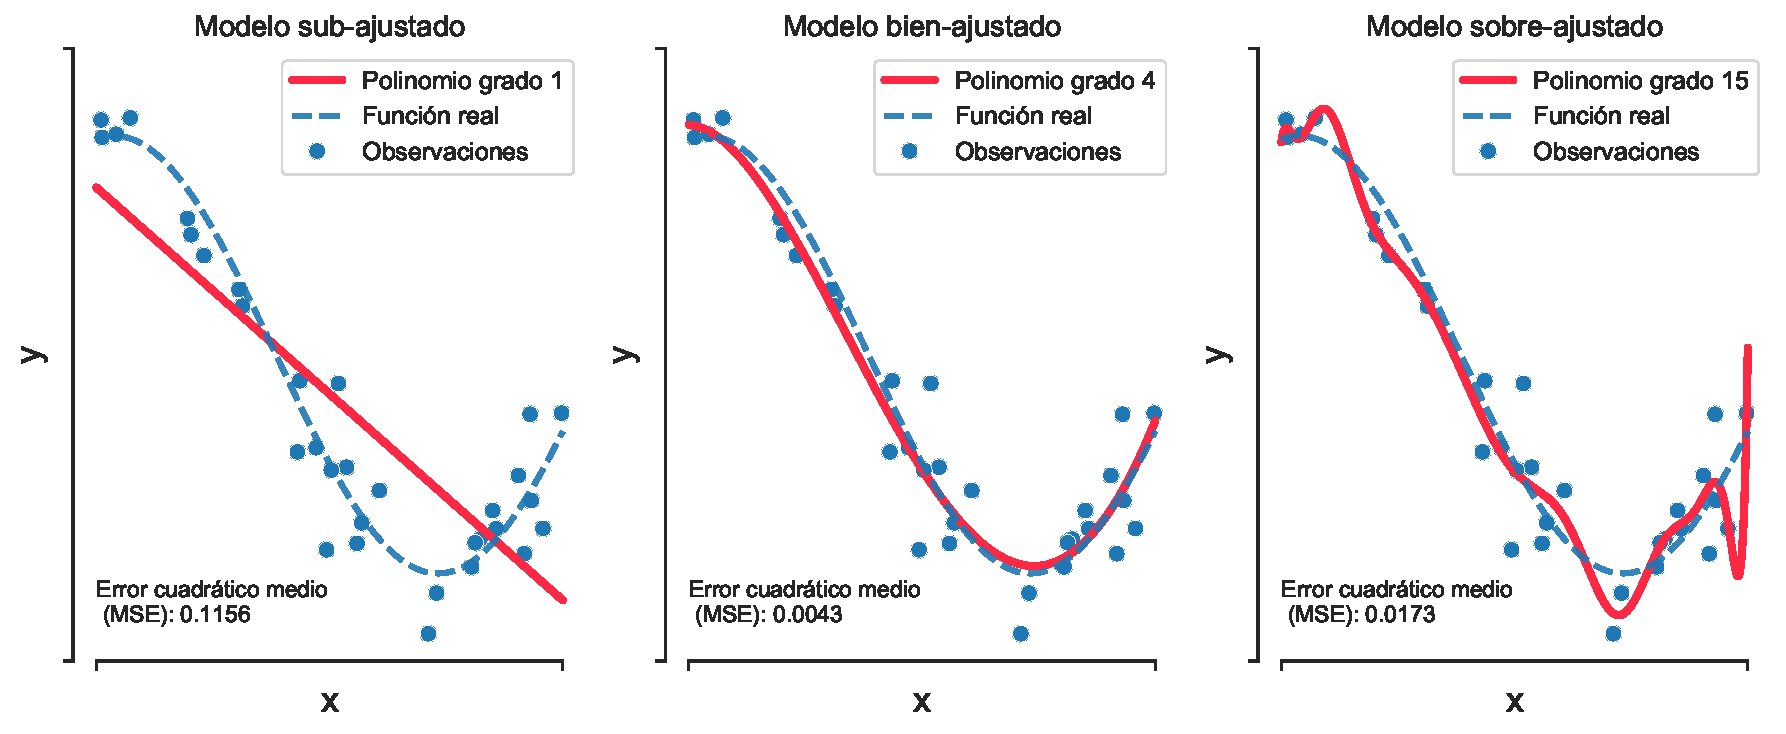
\includegraphics[width = 0.8\linewidth]{../img/cap4_ajuste.pdf}
\end{figure}\pause

El problema de sobreajuste puede ser observado al elegir el grado en una regresión polinomial ya que para $n$ puntos siempre existirá un polinomio de grado menor a $n$ que pase exactamente por dichos puntos, por lo que es posible tener un error de ajuste nulo en los datos de entrenamiento, pero con un alto error de predicción en datos no vistos.

\end{frame}

%Descomposición sesgo-varianza.
\begin{frame}{Descomposición sesgo-varianza}

En el capítulo de regresión se probó que, si bien MCR introduce sesgo en el estimador, también disminuye la varianza del regresor, lo cual resultaba en una disminución del error esperado. El objetivo de esta parte será estudiar la descomposición sesgo-varianza para un modelo general.\pause

\begin{definition}
	Sea $\datos=\{(x_i,y_i)\}_{i=1}^n\subset\R^N\times\R$ un conjunto de observaciones generadas por una función desconocida $f:\R^N\to\R$ mediante $y=f(x)+\epsilon$ donde $\epsilon$ es una v.a. (ruido) con $\E(\epsilon)=0$ y $\text{Var}(\epsilon)=\sigma^2$. Sea $\hat{f}(\cdot|\datos)$ un estimador de $f$ determinado a partir de $\datos$, entonces, se tienen las siguientes definiciones:
	
	\begin{itemize}
		\item Error (cuadrático) esperado: $\E\left((y-\hat{f}(x|\datos))^2\right)$.\pause
		\item Sesgo del estimador: $\text{Bias}(\hat{f}(x|D)):=\E(\hat{f}\left(x|\datos) - y\right) = \E(\hat{f}(x|\datos)) - f(x)$.\pause
		\item Varianza del estimador: $\text{Var}(\hat{f}(x|D)) = \E\left(\left(\hat{f}(x|\datos)-\E(\hat{f}(x|\datos))\right)^2\right)$.
		
	\end{itemize}
\end{definition}
	
\end{frame}

%Descomposición sesgo-varianza.
\begin{frame}{Descomposición sesgo-varianza}
	
	Bajo las definiciones anteriores, se tiene el siguiente teorema:

\begin{theorem}[descomposición sesgo-varianza] Sea $\hat{f}(x|\datos)$ un estimador de $f$, entonces:

\begin{equation*}
	\E\left((y-\hat{f}(x|\datos))^2\right) = \text{Bias}^2(\hat{f}(x|\datos)) + \text{Var}(\hat{f}(x|\datos)) + \sigma^2
\end{equation*}
	
\end{theorem}\pause

\begin{columns}

\begin{column}{0.6\textwidth}

\begin{itemize}
	\item la varianza intrínseca del ruido imposibilita realizar predicciones exactas bajo cualquier modelo aleatorio. \pause
	\item se puede introducir sesgo en el modelo con el fin de disminuir la varianza y viceversa.\pause
	\item La combinación sesgo-varianza crea un error total convexo tal como se puede observar en la figura.
\end{itemize}

\end{column}

\begin{column}{0.4\textwidth}

\begin{figure}[h]
    \centering
    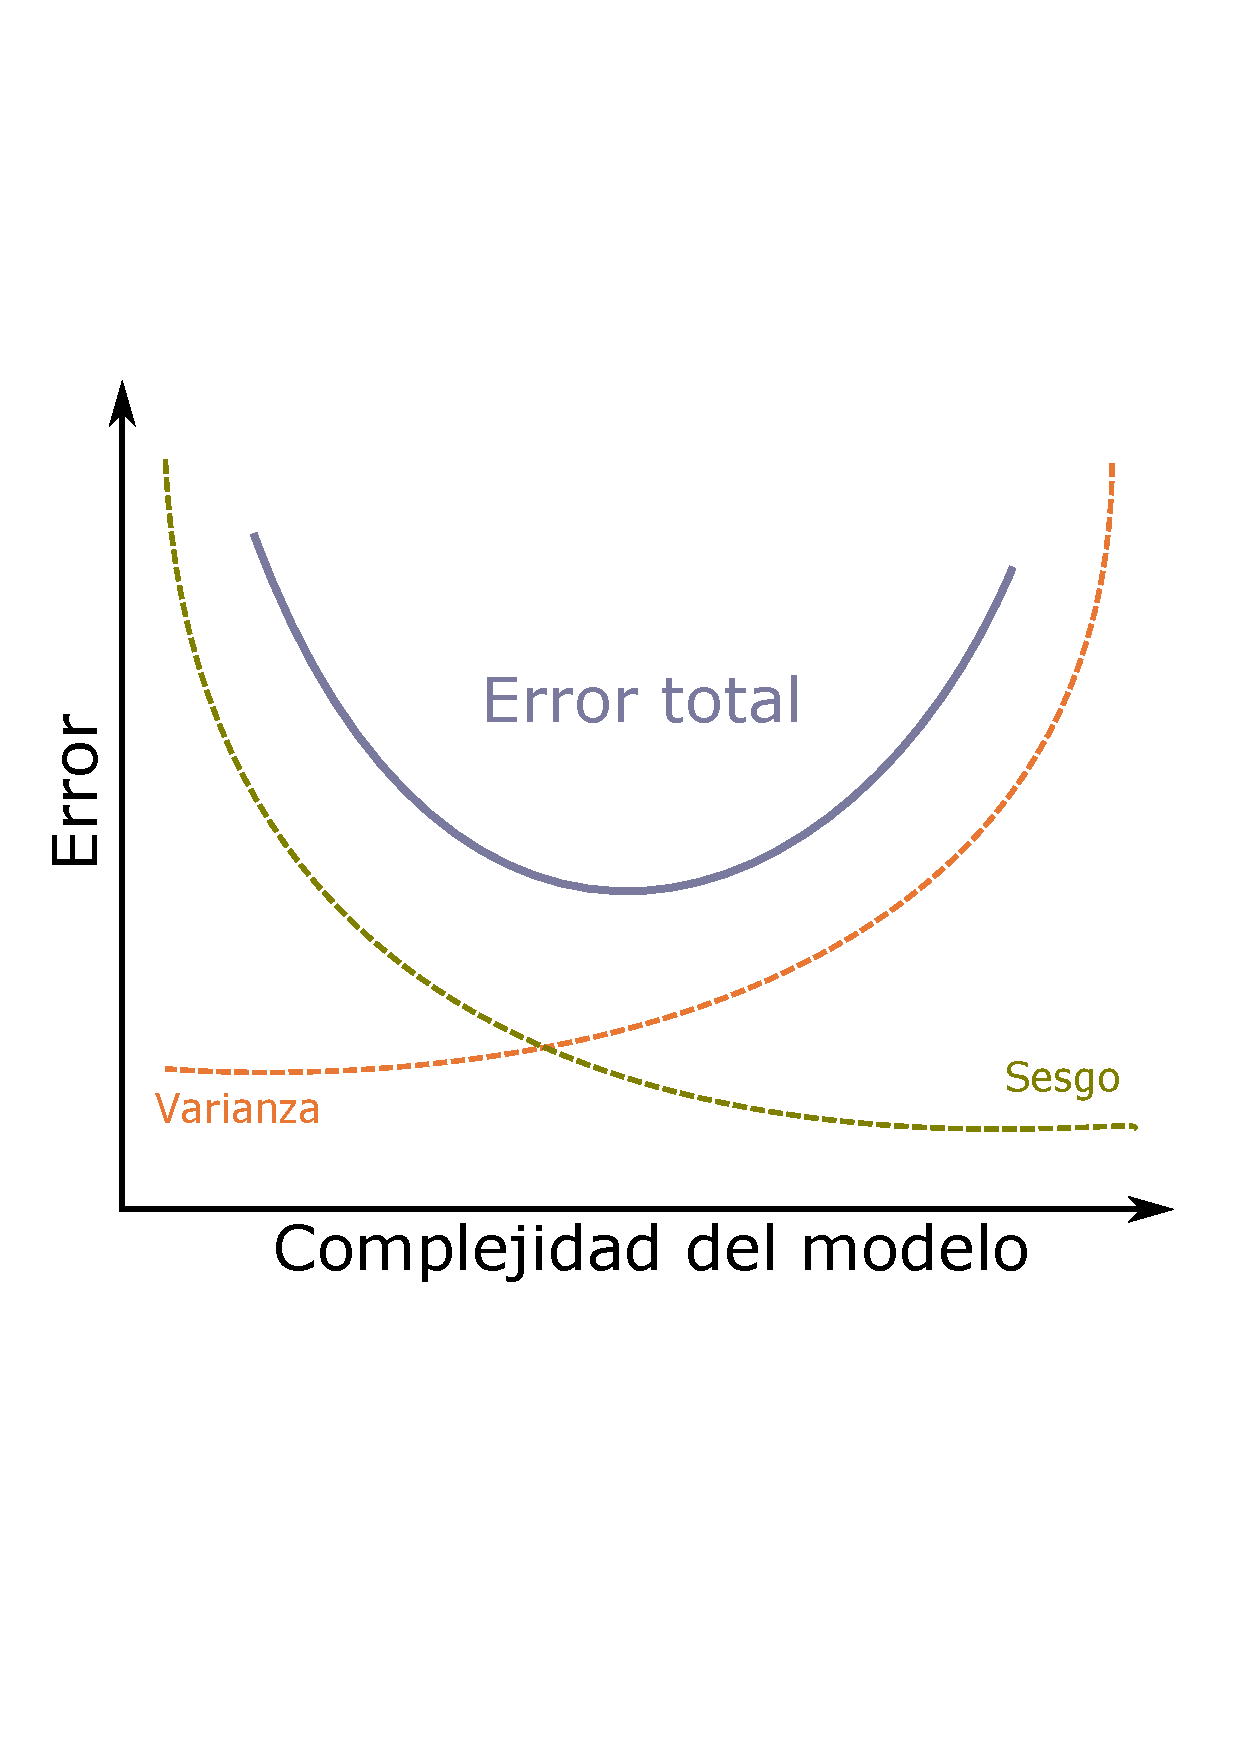
\includegraphics[width = \textwidth]{../img/cap4_biasvariance.pdf}
\end{figure}
\end{column}

\end{columns}\pause

Esto crea la pregunta acerca de cuál es el par sesgo-varianza óptimo que minimiza el error total (dilema sesgo-varianza).
	
\end{frame}

%Validación cruzada.
\begin{frame}{Validación cruzada}

Por lo general no se cuenta con la forma analítica del error cuadrático esperado como para poder elegir el mejor modelo. En estos casos, se vuelve necesario poder comparar modelos de forma relativa, utilizando el conjunto de datos $\datos$.\\~\ \pause

Una primera forma de elegir y evaluar un modelo fuera de muestra, consiste en particionar el conjunto de datos $\mathcal{D}$ en dos:

\begin{itemize}
	\item Conjunto de entrenamiento: se utilizará para entrenar el modelo.\pause
	\item Conjunto de validación: medirá el rendimiento del modelo de acuerdo a algún criterio predefinido (por ejemplo, ECM).\pause
\end{itemize}

Con el fin de evitar posibles sesgos provocados por una partición en específico, la evaluación de desempeño se debe realizar varias veces sobre conjuntos de validación distintos.\\~\ \pause

De esta forma, al promediar los rendimientos de cada partición se obtiene un rendimiento estimado fuera de muestra, lo cual permite finalmente elegir un modelo, quedándose con aquel que reporte el menor error out-sample.\\~\ \pause

Las distintas formas de mezclar y particionar los datos se conocen como \emph{validación cruzada}.
	
\end{frame}


%Validación cruzada exhaustiva.
\begin{frame}{Validación cruzada exhaustiva}

Un primer tipo de validación cruzada corresponde a CV exhaustiva. En este tipo de validación cruzada, se prueban todas las posibles permutaciones de los datos al particionar el conjunto $\mathcal{D}$. \pause Se tienen 2 técnicas exhaustivas:

\begin{itemize}
	\item \textbf{leave $p$ out (LpOCV):} el conjunto $\mathcal{D}$ se particiona dejando $p$ elementos para validación y los $N-p$ elementos restantes se utilizan para entrenar el modelo. Este entrenamiento y cálculo de desempeño se repite $C_p^N=\frac{N!}{(N-p)!p!}$ veces, pasando por todos los posibles conjuntos de validación de tamaño $p$. \pause
	\item \textbf{leave one out (LOOCV):} corresponde al caso anterior con $p=1$. En este caso cada dato de $\mathcal{D}$ es utilizado como único elemento de validación mientras el resto de los datos se utiliza para entrenar.
\end{itemize}

\end{frame}

%Validación cruzada no exhaustiva.
\begin{frame}{Validación cruzada no exhaustiva}
	
Por otra parte, existen dos tipos de validación cruzada no exhaustiva: \pause
	
\begin{itemize}
	\item \textbf{$k$-fold:} el conjunto $\mathcal{D}$ es dividido en $k$ grupos de igual tamaño. Luego, uno de esos grupos es utilizado como validador y el resto como entranemiento. Esto se repite $k$ veces de forma de que todos los grupos sean validadores una y solo una vez.\pause
	\item \textbf{Monte Carlo CV:} se realizan particiones binarias aleatorias de $\mathcal{D}$. Se entrena y evalúa usando el par de conjuntos creados en cada partición.
\end{itemize}

\end{frame}

%Variante de la validación cruzada.
\begin{frame}{Variante de la validación cruzada}

Una variante de la validación cruzada es dividir el conjunto $\datos$ en 3: \pause

\begin{itemize}
	\item Los primeros dos conjuntos son utilizados para entrenamiento y validación. \pause
	\item El tercer conjunto (conocido como test set) es utilizado para obtener una estimación real del desempeño fuera de muestra del modelo elegido a partir de los dos conjuntos anteriores. \pause
\end{itemize}

Esto se realiza ya que al considerar únicamente el desempeño en el conjunto de validación, por lo general se sobreestima el desempeño real fuera de muestra debido a que el modelo fue elegido precisamente tomando el que reporta el menor error dentro del conjunto de validación.\\~\ \pause

\textbf{Observación:} Si bien no hay una regla estándar que indique cómo particionar el conjunto, una división usual es utilizar el 50\% para entrenamiento y 25\% para validación y test.
	
\end{frame}


%Desventajas de la validación cruzada.
\begin{frame}{Desventajas de la validación cruzada}

Si bien la técnica de validación cruzada es bastante efectiva, tiene la limitación de requerir una gran cantidad de datos para poder realizar la partición de $\datos$.\\~\ 

Para los casos que en los que no se cuenta con una cantidad considerable de observaciones, se requieren herramientas más sofisticadas para poder tomar una decisión acerca de qué modelo elegir.\\~\ \pause

La próxima clase se estudiarán dos criterios para selección de modelos:

\begin{itemize}
	\item Criterio de información de Akaike (AIC).
	\item Criterio de información bayesiano (BIC).
\end{itemize}

	
\end{frame}



\end{document}
